

\tikzset{every picture/.style={line width=0.75pt}} %set default line width to 0.75pt        

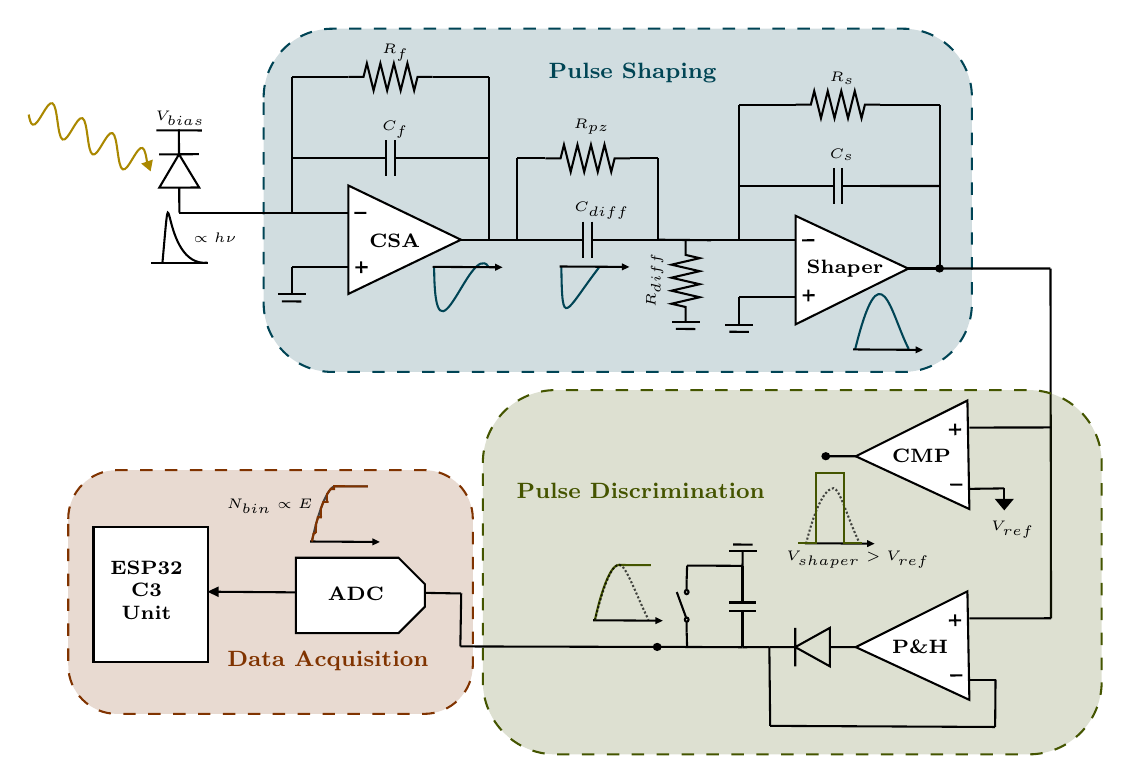
\begin{tikzpicture}[x=0.75pt,y=0.75pt,yscale=-1,xscale=1]
%uncomment if require: \path (0,390); %set diagram left start at 0, and has height of 390

%Rounded Rect [id:dp46800229916678826] 
\draw  [color={rgb, 255:red, 128; green, 51; blue, 0 }  ,draw opacity=1 ][fill={rgb, 255:red, 128; green, 51; blue, 0 }  ,fill opacity=0.18 ][dash pattern={on 4.5pt off 4.5pt}] (75.7,255.44) .. controls (75.7,242.46) and (86.22,231.95) .. (99.19,231.95) -- (247.14,231.95) .. controls (260.12,231.95) and (270.63,242.46) .. (270.63,255.44) -- (270.63,325.9) .. controls (270.63,338.88) and (260.12,349.39) .. (247.14,349.39) -- (99.19,349.39) .. controls (86.22,349.39) and (75.7,338.88) .. (75.7,325.9) -- cycle ;
%Rounded Rect [id:dp6060718292152891] 
\draw  [color={rgb, 255:red, 0; green, 68; blue, 85 }  ,draw opacity=1 ][fill={rgb, 255:red, 0; green, 68; blue, 85 }  ,fill opacity=0.18 ][dash pattern={on 4.5pt off 4.5pt}] (169.85,52.35) .. controls (169.85,34.09) and (184.66,19.28) .. (202.92,19.28) -- (478.01,19.28) .. controls (496.28,19.28) and (511.09,34.09) .. (511.09,52.35) -- (511.09,151.57) .. controls (511.09,169.84) and (496.28,184.64) .. (478.01,184.64) -- (202.92,184.64) .. controls (184.66,184.64) and (169.85,169.84) .. (169.85,151.57) -- cycle ;
%Straight Lines [id:da20418652663852965] 
\draw    (118.17,68.23) -- (140.04,68.31) ;
%Shape: Diode [id:dp9073484797643522] 
\draw   (119.56,95.88) -- (129.08,79.78) -- (138.77,95.78) -- (119.56,95.88) -- cycle (129.23,107.87) -- (129.17,95.83) (119.47,79.83) -- (138.68,79.73) (129.08,79.78) -- (129.01,67.74) ;
%Straight Lines [id:da29328469712985317] 
\draw    (129.23,107.87) -- (210.63,107.87) ;
%Shape: Triangle [id:dp7568885508488827] 
\draw  [fill={rgb, 255:red, 255; green, 255; blue, 255 }  ,fill opacity=1 ] (264.89,120.94) -- (210.63,147.08) -- (210.63,94.8) -- cycle ;
%Straight Lines [id:da4819348879555857] 
\draw    (210.63,134.01) -- (183.5,134.01) ;
%Straight Lines [id:da645749601403131] 
\draw    (183.5,147.08) -- (183.5,134.01) ;
%Straight Lines [id:da6803870332982462] 
\draw    (176.71,147.27) -- (190.28,147.27) ;
%Straight Lines [id:da005605298303441364] 
\draw    (178.65,150.63) -- (188.04,150.71) ;
%Straight Lines [id:da05308331089564988] 
\draw    (183.5,107.87) -- (183.5,81.73) ;
%Straight Lines [id:da020906030143946763] 
\draw    (183.5,42.51) -- (183.5,94.8) ;
%Shape: Resistor [id:dp7434947714198523] 
\draw   (210.63,42.51) -- (217.95,42.51) -- (219.58,35.98) -- (222.83,49.05) -- (226.09,35.98) -- (229.35,49.05) -- (232.6,35.98) -- (235.86,49.05) -- (239.11,35.98) -- (242.37,49.05) -- (244,42.51) -- (251.32,42.51) ;
%Shape: Capacitor [id:dp42145798620234975] 
\draw   (210.63,81.73) -- (228.94,81.73) (233.01,72.99) -- (233.01,90.46) (228.94,72.99) -- (228.94,90.46) (233.01,81.73) -- (251.32,81.73) ;
%Straight Lines [id:da34880193469214116] 
\draw    (210.63,42.51) -- (183.5,42.51) ;
%Straight Lines [id:da026503265572629386] 
\draw    (264.89,120.94) -- (292.02,120.94) ;
%Straight Lines [id:da9274117024294998] 
\draw    (278.45,42.51) -- (278.45,120.94) ;
%Straight Lines [id:da7747280381922488] 
\draw    (251.32,42.51) -- (278.45,42.51) ;
%Straight Lines [id:da1032408852686264] 
\draw    (183.5,81.73) -- (210.63,81.73) ;
%Straight Lines [id:da1423279487465121] 
\draw    (251.32,81.73) -- (278.45,81.73) ;
%Curve Lines [id:da7997259707368105] 
\draw [color={rgb, 255:red, 0; green, 0; blue, 0 }  ,draw opacity=1 ][fill={rgb, 255:red, 255; green, 255; blue, 255 }  ,fill opacity=1 ]   (121.09,132.03) .. controls (126.11,76.56) and (119.49,134.29) .. (142.8,132.03) ;
%Straight Lines [id:da9485003249156622] 
\draw    (115.67,132.03) -- (142.8,132.03) ;
%Curve Lines [id:da49583939836969093] 
\draw [color={rgb, 255:red, 0; green, 68; blue, 85 }  ,draw opacity=1 ]   (313.29,133.84) .. controls (313.63,164.72) and (314.85,155.96) .. (331.36,134.4) ;
%Shape: Resistor [id:dp18008683636522793] 
\draw   (305.58,81.73) -- (312.91,81.73) -- (314.54,75.19) -- (317.79,88.26) -- (321.05,75.19) -- (324.3,88.26) -- (327.56,75.19) -- (330.81,88.26) -- (334.07,75.19) -- (337.33,88.26) -- (338.95,81.73) -- (346.28,81.73) ;
%Straight Lines [id:da6245327821504196] 
\draw    (292.02,120.94) -- (292.02,81.73) ;
%Straight Lines [id:da9330542602485921] 
\draw    (292.02,81.73) -- (305.58,81.73) ;
%Straight Lines [id:da7057152830278173] 
\draw    (292.02,120.94) -- (305.58,120.94) ;
%Shape: Capacitor [id:dp8095550086511366] 
\draw   (305.58,120.94) -- (323.9,120.94) (327.97,112.21) -- (327.97,129.67) (323.9,112.21) -- (323.9,129.67) (327.97,120.94) -- (346.28,120.94) ;
%Straight Lines [id:da5386226934871385] 
\draw    (346.28,81.73) -- (359.84,81.73) ;
%Straight Lines [id:da7313083657794016] 
\draw    (346.28,120.94) -- (359.84,120.94) ;
%Straight Lines [id:da03131911441569635] 
\draw    (359.84,81.73) -- (359.84,120.94) ;
%Curve Lines [id:da7413273067238557] 
\draw [color={rgb, 255:red, 0; green, 68; blue, 85 }  ,draw opacity=1 ][line width=0.75]    (252,134.01) .. controls (252.17,187.85) and (269.17,121.74) .. (278,133.68) ;
%Shape: Triangle [id:dp6184826935280519] 
\draw  [fill={rgb, 255:red, 255; green, 255; blue, 255 }  ,fill opacity=1 ] (480.43,134.86) -- (426.17,161.72) -- (426.17,109.44) -- cycle ;
%Straight Lines [id:da31773246729249327] 
\draw    (426.17,148.65) -- (399.03,148.65) ;
%Straight Lines [id:da3550332613541024] 
\draw    (399.03,161.72) -- (399.03,148.65) ;
%Straight Lines [id:da8025351063037379] 
\draw    (392.25,161.91) -- (405.82,161.91) ;
%Straight Lines [id:da02403217066549712] 
\draw    (394.19,165.27) -- (403.58,165.35) ;
%Straight Lines [id:da16841076045424963] 
\draw    (385.47,121.2) -- (426.17,121.2) ;
%Straight Lines [id:da5746709989474186] 
\draw    (399.03,121.2) -- (399.03,95.06) ;
%Straight Lines [id:da2718623980119098] 
\draw    (399.03,55.84) -- (399.03,108.13) ;
%Shape: Resistor [id:dp29501269522921625] 
\draw   (426.17,55.84) -- (433.49,55.84) -- (435.12,49.31) -- (438.37,62.38) -- (441.63,49.31) -- (444.89,62.38) -- (448.14,49.31) -- (451.4,62.38) -- (454.65,49.31) -- (457.91,62.38) -- (459.54,55.84) -- (466.86,55.84) ;
%Shape: Capacitor [id:dp6295648569904636] 
\draw   (426.17,95.06) -- (444.48,95.06) (448.55,86.32) -- (448.55,103.79) (444.48,86.32) -- (444.48,103.79) (448.55,95.06) -- (466.86,95.06) ;
%Straight Lines [id:da39447831240426734] 
\draw    (426.17,55.84) -- (399.03,55.84) ;
%Straight Lines [id:da7401181488947025] 
\draw    (548.94,134.81) -- (549.21,303.33) ;
%Straight Lines [id:da3780881206944031] 
\draw    (466.86,55.84) -- (495.5,55.84) ;
%Straight Lines [id:da4232645895231355] 
\draw    (399.03,95.06) -- (426.17,95.06) ;
%Straight Lines [id:da4266027647624573] 
\draw    (466.86,95.06) -- (495.95,95.05) ;
%Straight Lines [id:da5672944700293289] 
\draw    (480.43,134.8) -- (495.5,134.8) ;
%Straight Lines [id:da469893720694727] 
\draw    (213.52,108.04) -- (219.36,107.98) ;
%Straight Lines [id:da9392787125105846] 
\draw    (251.32,134.01) -- (281.93,134.21) ;
\draw [shift={(284.93,134.23)}, rotate = 180.37] [fill={rgb, 255:red, 0; green, 0; blue, 0 }  ][line width=0.08]  [draw opacity=0] (3.57,-1.72) -- (0,0) -- (3.57,1.72) -- cycle    ;
%Straight Lines [id:da6932257001220354] 
\draw    (312.44,133.84) -- (343.05,134.03) ;
\draw [shift={(346.05,134.05)}, rotate = 180.37] [fill={rgb, 255:red, 0; green, 0; blue, 0 }  ][line width=0.08]  [draw opacity=0] (3.57,-1.72) -- (0,0) -- (3.57,1.72) -- cycle    ;
%Straight Lines [id:da6166140138845793] 
\draw    (214.06,134.25) -- (219.9,134.19) ;
%Shape: Boxed Line [id:dp7328235768970041] 
\draw    (216.82,131.4) -- (216.87,137.02) ;
%Straight Lines [id:da9592107478171705] 
\draw    (429.33,121.24) -- (435.17,121.18) ;
%Shape: Boxed Line [id:dp06578186279615383] 
\draw    (432.26,145) -- (432.31,150.63) ;
%Straight Lines [id:da21273186496269592] 
\draw    (429.48,147.76) -- (435.31,147.69) ;
%Shape: Resistor [id:dp07090411488435666] 
\draw   (373.14,121.2) -- (373.14,128.26) -- (379.92,129.83) -- (366.35,132.97) -- (379.92,136.1) -- (366.35,139.24) -- (379.92,142.38) -- (366.35,145.51) -- (379.92,148.65) -- (366.35,151.79) -- (373.14,153.36) -- (373.14,160.42) ;
%Straight Lines [id:da5181129573733605] 
\draw    (366.56,160.54) -- (380.13,160.54) ;
%Straight Lines [id:da36868876671547046] 
\draw    (368.5,163.9) -- (377.89,163.98) ;
%Straight Lines [id:da4086711222947753] 
\draw    (359.84,120.94) -- (385.47,121.2) ;
%Rounded Rect [id:dp3460824200505386] 
\draw  [color={rgb, 255:red, 68; green, 85; blue, 0 }  ,draw opacity=1 ][fill={rgb, 255:red, 68; green, 85; blue, 0 }  ,fill opacity=0.18 ][dash pattern={on 4.5pt off 4.5pt}] (275.46,228.49) .. controls (275.46,209.1) and (291.18,193.39) .. (310.56,193.39) -- (538.52,193.39) .. controls (557.91,193.39) and (573.62,209.1) .. (573.62,228.49) -- (573.62,333.79) .. controls (573.62,353.18) and (557.91,368.89) .. (538.52,368.89) -- (310.56,368.89) .. controls (291.18,368.89) and (275.46,353.18) .. (275.46,333.79) -- cycle ;
%Shape: Triangle [id:dp21057859356469377] 
\draw  [fill={rgb, 255:red, 255; green, 255; blue, 255 }  ,fill opacity=1 ] (455.14,225.28) -- (508.92,198.42) -- (509.87,250.71) -- cycle ;
%Straight Lines [id:da7294664906139928] 
\draw    (506.48,238.91) -- (500.65,238.97) ;
%Shape: Boxed Line [id:dp3537895946781868] 
\draw    (503.13,215.14) -- (502.98,209.52) ;
%Straight Lines [id:da9669577971099538] 
\draw    (505.86,212.39) -- (500.02,212.45) ;
%Straight Lines [id:da8006808934622864] 
\draw    (510.26,240.97) -- (526.57,240.75) ;
%Shape: Triangle [id:dp4851626389643716] 
\draw  [fill={rgb, 255:red, 0; green, 0; blue, 0 }  ,fill opacity=1 ] (526.69,250.57) -- (523.14,246.29) -- (530.24,246.29) -- cycle ;
%Straight Lines [id:da7399314250868523] 
\draw    (455.14,225.28) -- (440.69,225.25) ;
%Flowchart: Connector [id:dp3531466314065995] 
\draw  [fill={rgb, 255:red, 0; green, 0; blue, 0 }  ,fill opacity=1 ] (493.88,134.8) .. controls (493.88,134) and (494.61,133.35) .. (495.5,133.35) .. controls (496.39,133.35) and (497.11,134) .. (497.11,134.8) .. controls (497.11,135.59) and (496.39,136.24) .. (495.5,136.24) .. controls (494.61,136.24) and (493.88,135.59) .. (493.88,134.8) -- cycle ;
%Straight Lines [id:da9446115204522941] 
\draw    (509.88,211.45) -- (549.21,211.39) ;
%Curve Lines [id:da31175352604231354] 
\draw [color={rgb, 255:red, 0; green, 68; blue, 85 }  ,draw opacity=1 ]   (454.82,173.8) .. controls (467.17,123.88) and (471.61,155.96) .. (480.63,173.55) ;
%Straight Lines [id:da8734375505712497] 
\draw    (453.91,173.8) -- (484.52,174) ;
\draw [shift={(487.51,174.02)}, rotate = 180.37] [fill={rgb, 255:red, 0; green, 0; blue, 0 }  ][line width=0.08]  [draw opacity=0] (3.57,-1.72) -- (0,0) -- (3.57,1.72) -- cycle    ;
%Straight Lines [id:da6007611642847911] 
\draw    (430.57,267.17) -- (461.17,267.37) ;
\draw [shift={(464.17,267.38)}, rotate = 180.37] [fill={rgb, 255:red, 0; green, 0; blue, 0 }  ][line width=0.08]  [draw opacity=0] (3.57,-1.72) -- (0,0) -- (3.57,1.72) -- cycle    ;
%Curve Lines [id:da5409343504904985] 
\draw [color={rgb, 255:red, 0; green, 0; blue, 0 }  ,draw opacity=0.7 ] [dash pattern={on 0.75pt off 0.75pt on 0.75pt off 0.75pt}]  (431.19,267.37) .. controls (436.14,247.38) and (441.17,240.57) .. (444.39,240.68) .. controls (447.6,240.8) and (451.6,256.57) .. (457.01,267.12) ;
%Shape: Pulse Wave Form [id:dp37814170861699237] 
\draw  [color={rgb, 255:red, 68; green, 85; blue, 0 }  ,draw opacity=1 ] (427.44,267.23) -- (435.91,267.23) -- (435.91,233.36) -- (449.48,233.36) -- (449.48,267.23) -- (457.96,267.23) ;

%Straight Lines [id:da8033158731026477] 
\draw    (328.55,304.29) -- (359.16,304.48) ;
\draw [shift={(362.16,304.5)}, rotate = 180.37] [fill={rgb, 255:red, 0; green, 0; blue, 0 }  ][line width=0.08]  [draw opacity=0] (3.57,-1.72) -- (0,0) -- (3.57,1.72) -- cycle    ;
%Curve Lines [id:da8165839321439692] 
\draw [color={rgb, 255:red, 68; green, 85; blue, 0 }  ,draw opacity=1 ]   (329.46,304.29) .. controls (330.89,296.83) and (335.71,278.62) .. (340.54,277.66) ;
%Straight Lines [id:da9249993527350234] 
\draw [color={rgb, 255:red, 68; green, 85; blue, 0 }  ,draw opacity=1 ]   (340.54,277.66) -- (356.36,277.74) ;
%Curve Lines [id:da01278581006202073] 
\draw [color={rgb, 255:red, 0; green, 0; blue, 0 }  ,draw opacity=0.7 ] [dash pattern={on 0.75pt off 0.75pt on 0.75pt off 0.75pt}]  (329.46,304.29) .. controls (334.41,284.3) and (338.09,277.46) .. (341.3,277.57) .. controls (344.51,277.68) and (349.87,293.49) .. (355.27,304.04) ;
%Straight Lines [id:da36645697031500035] 
\draw    (526.57,245.78) -- (526.57,240.75) ;
%Shape: Triangle [id:dp48501946316287736] 
\draw  [fill={rgb, 255:red, 255; green, 255; blue, 255 }  ,fill opacity=1 ] (455.14,317.22) -- (508.92,290.36) -- (509.87,342.64) -- cycle ;
%Straight Lines [id:da6036906170346914] 
\draw    (506.48,330.84) -- (500.65,330.91) ;
%Shape: Boxed Line [id:dp6726482576478763] 
\draw    (503.13,307.08) -- (502.98,301.45) ;
%Straight Lines [id:da037444841152633135] 
\draw    (505.86,304.32) -- (500.02,304.39) ;
%Straight Lines [id:da5709459533271122] 
\draw    (510.26,332.91) -- (522.47,332.91) ;
%Straight Lines [id:da19356976941121384] 
\draw    (509.88,303.38) -- (549.21,303.33) ;
%Shape: Diode [id:dp614316518769653] 
\draw   (442.65,326.48) -- (425.99,317.22) -- (442.65,307.96) -- (442.65,326.48) -- cycle (455.14,317.22) -- (442.65,317.22) (425.99,326.48) -- (425.99,307.96) (425.99,317.22) -- (413.5,317.22) ;
%Straight Lines [id:da09813703953082598] 
\draw    (413.5,317.22) -- (413.9,355.16) ;
%Straight Lines [id:da849214487415646] 
\draw    (413.9,355.16) -- (522.28,355.7) ;
%Straight Lines [id:da125511136072201] 
\draw    (522.47,332.91) -- (522.28,355.7) ;
%Shape: Capacitor [id:dp7142356900456059] 
\draw   (400.56,278.07) -- (400.56,295.71) (407,299.63) -- (394.12,299.63) (407,295.71) -- (394.12,295.71) (400.56,299.63) -- (400.56,317.28) ;
%Shape: Simple Switch [id:dp5297728261178234] 
\draw   (373.67,310.11) -- (373.67,305) (373.67,289.68) -- (373.67,284.57) (373.37,302.96) -- (368.9,290.7) (373.67,291.72) .. controls (373.18,291.72) and (372.78,291.26) .. (372.78,290.7) .. controls (372.78,290.14) and (373.18,289.68) .. (373.67,289.68) .. controls (374.17,289.68) and (374.57,290.14) .. (374.57,290.7) .. controls (374.57,291.26) and (374.17,291.72) .. (373.67,291.72) -- cycle (373.67,305) .. controls (373.18,305) and (372.78,304.54) .. (372.78,303.98) .. controls (372.78,303.42) and (373.18,302.96) .. (373.67,302.96) .. controls (374.17,302.96) and (374.57,303.42) .. (374.57,303.98) .. controls (374.57,304.54) and (374.17,305) .. (373.67,305) -- cycle ;
%Straight Lines [id:da9962880185364887] 
\draw    (400.56,278.07) -- (373.87,277.93) ;
%Straight Lines [id:da4168400592441782] 
\draw    (400.56,317.28) -- (373.87,317.15) ;
%Straight Lines [id:da6629627230865746] 
\draw    (373.87,277.93) -- (373.67,284.57) ;
%Straight Lines [id:da6227335867281195] 
\draw    (373.67,310.11) -- (373.87,317.15) ;
%Straight Lines [id:da9440197749138511] 
\draw    (400.56,317.28) -- (413.5,317.22) ;
%Straight Lines [id:da5574398837436616] 
\draw    (373.87,317.15) -- (359.47,317.14) ;
%Flowchart: Connector [id:dp28586564232252365] 
\draw  [fill={rgb, 255:red, 0; green, 0; blue, 0 }  ,fill opacity=1 ] (439.08,225.25) .. controls (439.08,224.45) and (439.8,223.81) .. (440.69,223.81) .. controls (441.58,223.81) and (442.3,224.45) .. (442.3,225.25) .. controls (442.3,226.05) and (441.58,226.69) .. (440.69,226.69) .. controls (439.8,226.69) and (439.08,226.05) .. (439.08,225.25) -- cycle ;
%Flowchart: Connector [id:dp5135507227534388] 
\draw  [fill={rgb, 255:red, 0; green, 0; blue, 0 }  ,fill opacity=1 ] (357.86,317.14) .. controls (357.86,316.35) and (358.58,315.7) .. (359.47,315.7) .. controls (360.36,315.7) and (361.08,316.35) .. (361.08,317.14) .. controls (361.08,317.94) and (360.36,318.58) .. (359.47,318.58) .. controls (358.58,318.58) and (357.86,317.94) .. (357.86,317.14) -- cycle ;
%Shape: Wave [id:dp059927494842615836] 
\draw  [color={rgb, 255:red, 170; green, 136; blue, 0 }  ,draw opacity=1 ] (56.66,60.65) .. controls (57.1,63.11) and (57.63,65.03) .. (58.51,65.46) .. controls (59.82,66.11) and (61.52,63.3) .. (63.3,60.33) .. controls (65.08,57.37) and (66.78,54.56) .. (68.09,55.21) .. controls (69.4,55.86) and (69.96,59.8) .. (70.54,63.93) .. controls (71.12,68.06) and (71.67,72) .. (72.98,72.65) .. controls (74.29,73.3) and (75.99,70.48) .. (77.77,67.52) .. controls (79.55,64.56) and (81.25,61.75) .. (82.56,62.4) .. controls (83.87,63.05) and (84.43,66.98) .. (85,71.12) .. controls (85.58,75.25) and (86.14,79.19) .. (87.45,79.84) .. controls (88.76,80.49) and (90.46,77.67) .. (92.24,74.71) .. controls (94.02,71.75) and (95.72,68.94) .. (97.03,69.59) .. controls (98.34,70.24) and (98.89,74.17) .. (99.47,78.31) .. controls (100.05,82.44) and (100.61,86.38) .. (101.92,87.03) .. controls (103.23,87.68) and (104.93,84.86) .. (106.71,81.9) .. controls (108.49,78.94) and (110.19,76.12) .. (111.5,76.77) .. controls (112.71,77.37) and (113.27,80.78) .. (113.81,84.55) ;
%Shape: Triangle [id:dp3108622029974263] 
\draw  [color={rgb, 255:red, 170; green, 136; blue, 0 }  ,draw opacity=1 ][fill={rgb, 255:red, 170; green, 136; blue, 0 }  ,fill opacity=1 ] (115.05,87.07) -- (111.86,84.44) -- (115.81,83.09) -- cycle ;
%Straight Lines [id:da5842921754561695] 
\draw    (400.56,278.07) -- (400.66,271.23) ;
%Straight Lines [id:da97191101904161] 
\draw    (396,267.77) -- (400.92,267.81) -- (405.39,267.84) ;
%Straight Lines [id:da8202699426795026] 
\draw    (393.99,271.03) -- (395.72,271.03) -- (407.56,271.03) ;
%Snip Same Side Corner Rect [id:dp24267720786095204] 
\draw  [fill={rgb, 255:red, 255; green, 255; blue, 255 }  ,fill opacity=1 ] (234.8,274.15) -- (247.52,286.87) -- (247.52,297.77) -- (234.8,310.49) -- (185.39,310.49) -- (185.39,310.49) -- (185.39,274.15) -- (185.39,274.15) -- cycle ;
%Shape: Rectangle [id:dp4960716974860516] 
\draw  [fill={rgb, 255:red, 255; green, 255; blue, 255 }  ,fill opacity=1 ] (87.86,259.38) -- (142.94,259.38) -- (142.94,324.22) -- (87.86,324.22) -- cycle ;
%Straight Lines [id:da5259235282088736] 
\draw    (264.62,316.89) -- (359.47,317.14) ;
%Straight Lines [id:da04918323557857496] 
\draw    (247.85,291.09) -- (265.04,291.38) ;
%Straight Lines [id:da700345769463564] 
\draw    (265.04,291.38) -- (264.62,316.89) ;
%Straight Lines [id:da44513384727711636] 
\draw    (192.21,266.34) -- (222.82,266.54) ;
\draw [shift={(225.82,266.56)}, rotate = 180.37] [fill={rgb, 255:red, 0; green, 0; blue, 0 }  ][line width=0.08]  [draw opacity=0] (3.57,-1.72) -- (0,0) -- (3.57,1.72) -- cycle    ;
%Curve Lines [id:da06577028557977793] 
\draw [color={rgb, 255:red, 0; green, 0; blue, 0 }  ,draw opacity=0.7 ]   (193.12,266.34) .. controls (194.55,258.88) and (199.36,240.67) .. (204.19,239.71) ;
%Straight Lines [id:da0572237289311508] 
\draw [color={rgb, 255:red, 0; green, 0; blue, 0 }  ,draw opacity=0.7 ]   (204.19,239.71) -- (220.01,239.8) ;
%Curve Lines [id:da3804043288541633] 
\draw [color={rgb, 255:red, 128; green, 51; blue, 0 }  ,draw opacity=1 ] [dash pattern={on 3pt off 3pt on 3pt off 3pt}]  (193.12,266.34) .. controls (194.55,258.88) and (199.36,240.67) .. (204.19,239.71) ;
%Straight Lines [id:da5333998307295363] 
\draw [color={rgb, 255:red, 128; green, 51; blue, 0 }  ,draw opacity=1 ]   (193.63,262.21) -- (195,262.32) ;
%Straight Lines [id:da40393427405433224] 
\draw [color={rgb, 255:red, 128; green, 51; blue, 0 }  ,draw opacity=1 ]   (195,262.32) -- (195.08,258.23) ;
%Straight Lines [id:da3824884565346163] 
\draw [color={rgb, 255:red, 128; green, 51; blue, 0 }  ,draw opacity=1 ]   (202.04,241.08) -- (204.32,241.09) ;
%Straight Lines [id:da8760345808356574] 
\draw [color={rgb, 255:red, 128; green, 51; blue, 0 }  ,draw opacity=1 ]   (203.75,241.36) -- (203.75,239.04) ;

%Straight Lines [id:da012864593156911797] 
\draw [color={rgb, 255:red, 128; green, 51; blue, 0 }  ,draw opacity=1 ]   (195.47,254.61) -- (197.96,254.68) ;
%Straight Lines [id:da7563678124476333] 
\draw [color={rgb, 255:red, 128; green, 51; blue, 0 }  ,draw opacity=1 ]   (197.4,255.23) -- (197.4,250.54) ;
%Straight Lines [id:da5333243365793827] 
\draw [color={rgb, 255:red, 128; green, 51; blue, 0 }  ,draw opacity=1 ]   (198.85,247.27) -- (198.18,247.22) -- (201.13,247.28) ;
%Straight Lines [id:da6175946543817453] 
\draw [color={rgb, 255:red, 128; green, 51; blue, 0 }  ,draw opacity=1 ]   (200.56,247.82) -- (200.56,247.22) -- (200.56,243.14) ;
%Straight Lines [id:da3521344691026579] 
\draw [color={rgb, 255:red, 128; green, 51; blue, 0 }  ,draw opacity=1 ]   (204.19,239.71) -- (220.01,239.8) ;
%Straight Lines [id:da18368526561352316] 
\draw    (185.87,290.85) -- (145.8,290.54) ;
\draw [shift={(142.8,290.52)}, rotate = 0.43] [fill={rgb, 255:red, 0; green, 0; blue, 0 }  ][line width=0.08]  [draw opacity=0] (5.36,-2.57) -- (0,0) -- (5.36,2.57) -- cycle    ;
%Straight Lines [id:da56033182920969] 
\draw    (495.5,55.84) -- (495.5,133.35) ;
%Straight Lines [id:da784442544187718] 
\draw    (495.5,134.8) -- (548.94,134.81) ;

% Text Node
\draw (225.47,25.29) node [anchor=north west][inner sep=0.75pt]  [font=\tiny] [align=left] {$R_{f}$};
% Text Node
\draw (225.47,62.28) node [anchor=north west][inner sep=0.75pt]  [font=\tiny] [align=left] {$C_{f}$};
% Text Node
\draw (116.3,57.49) node [anchor=north west][inner sep=0.75pt]  [font=\tiny] [align=left] {$V_{bias}$};
% Text Node
\draw (134.54,116.18) node [anchor=north west][inner sep=0.75pt] [font=\tiny] {\(\propto h\nu\)};
% Text Node
\draw (317.75,61.5) node [anchor=north west][inner sep=0.75pt]  [font=\tiny] [align=left] {$R_{pz}$};
% Text Node
\draw (318.11,101.49) node [anchor=north west][inner sep=0.75pt]  [font=\tiny] [align=left] {$C_{diff}$};
% Text Node
\draw (441.01,38.62) node [anchor=north west][inner sep=0.75pt]  [font=\tiny] [align=left] {$R_{s}$};
% Text Node
\draw (441.01,75.61) node [anchor=north west][inner sep=0.75pt]  [font=\tiny] [align=left] {$C_{s}$};
% Text Node
\draw (219.33,116.63) node [anchor=north west][inner sep=0.75pt]  [font=\scriptsize] [align=left] {{\scriptsize \textbf{CSA}}};
% Text Node
\draw (430,129) node [anchor=north west][inner sep=0.75pt]  [font=\scriptsize] [align=left] {{\scriptsize \textbf{Shaper}}};
% Text Node
\draw (305.69,34.53) node [anchor=north west][inner sep=0.75pt]   [align=left] {\textbf{{\footnotesize \textcolor[rgb]{0,0.27,0.33}{Pulse Shaping}}}};
% Text Node
\draw (352.68,155.01) node [anchor=north west][inner sep=0.75pt]  [font=\tiny,rotate=-270] [align=left] {$R_{diff}$};
% Text Node
\draw (518.87,255.11) node [anchor=north west][inner sep=0.75pt]  [font=\tiny] [align=left] {$V_{ref}$};
% Text Node
\draw (471.18,220.38) node [anchor=north west][inner sep=0.75pt]  [font=\scriptsize] [align=left] {{\scriptsize \textbf{CMP}}};
% Text Node
\draw (420.26,269.33) node [anchor=north west][inner sep=0.75pt]   [align=left] {{\tiny $V_{shaper} > V_{ref}$}};
% Text Node
\draw (471.18,312.13) node [anchor=north west][inner sep=0.75pt]  [font=\scriptsize] [align=left] {{\scriptsize \textbf{P\&H}}};
% Text Node
\draw (290.23,236.5) node [anchor=north west][inner sep=0.75pt]   [align=left] {\textbf{{\footnotesize \textcolor[rgb]{0.27,0.33,0}{Pulse Discrimination}}}};
% Text Node
\draw (199.34,286.87) node [anchor=north west][inner sep=0.75pt]  [font=\scriptsize] [align=left] {{\scriptsize \textbf{ADC}}};
% Text Node
\draw (94.49,274.48) node [anchor=north west][inner sep=0.75pt] [font=\scriptsize] [align=center] {
\textbf{ESP32}\\
\textbf{C3}\\
\textbf{Unit}
};
% Text Node
\draw (150.9,317.64) node [anchor=north west][inner sep=0.75pt]   [align=left] {\textbf{{\footnotesize \textcolor[rgb]{0.5,0.2,0}{Data Acquisition}}}};
% Text Node
\draw (150.67,244.28) node [anchor=north west][inner sep=0.75pt]  [font=\tiny] [align=left] {$N_{\text{bin}} \propto E$};

\end{tikzpicture}


